\documentclass[a4paper,12pt,oneside]{report}%FinalView
%\documentclass[draft,a4paper,12pt,oneside]{report}%draftView

\input{settings/preamble.tex}%Inputs Preamble for its .tex
\usepackage[color]{showkeys}%Shows cross ref paths

\begin{document}

%%%%%%%%%%%%%%%%%%%%%%%%%%%%%%%%%%%%%%%%%%%%%%%%%%%%%%%%%%%%%%%%%%%%%%%%%%

%Table of Contents
\tableofcontents\newpage
\addcontentsline{toc}{chapter}{TABLE OF CONTENTS}
\let\cleardoublepage\clearpage

%%%%%%%%%%%%%%%%%%%%%%%%%%%%%%%%%%%%%%%%%%%%%%%%%%%%%%%%%%%%%%%%%%%%%%%%%%

\chapter{EXPERIMENTAL PROCEDURE}

\section{Master Alloy}
The production of all bulk and film samples required master alloy of appropriate composition for the desired stoichiometry of \MgZnCa. These master alloy were produced by induction melting of pure constituent element ingots.

\subsection{Base Elements}
The master alloy of \MgZnCa~ was produced using high-purity elements of Mg (99.85 wt\%), Zn (99.995 wt\%), and Ca (99.8 wt\%). Each element ingot was linished or otherwise mechanically abraded to removal surface contamination and oxides. The ingots were cut to size on either a Struers Labotom-3 or a Struers Discotom-6 auto-cutter at a feed rate of no more than $0.2~ mm/s$ at $2850 - 3420$ \acrshort{rpm} (Figures \ref{fig:AutoCutter} and \ref{fig:MgIngot}).

%code to put 2 images side by side in a figure
\begin{figure}[htbp]
	\centering
	%Image 1
	\begin{subfigure}[htbp]{0.49\textwidth}
		\includegraphics[width=\textwidth]{Ex_AutoCutter.jpg}
		\caption{}
		\label{fig:AutoCutter}
	\end{subfigure}
	%Image 2
	\begin{subfigure}[htbp]{0.30\textwidth}
		\includegraphics[width=\textwidth]{Ex_Mg_Cut_Ingot.jpg}
		\caption{}
		\label{fig:MgIngot}
	\end{subfigure}
	\caption{(a) Struers Discotom-6 auto-cutter. (b) Cut and fully deoxided Mg ingot ready for casting.}%global caption
	\label{fig:Cutter_MgIngot}
\end{figure}

The total weight of each constituent element required for a master alloy charge was automatically calculated by a developed MS Excel workbook, Figure \ref{fig:ChargeSheet}. This tool auto-computes the required weights of each element from the prepared ingot innovatory, checks the expected master alloy composition, and provides a space for notes on the entire process (i.e. heating cycles, observations, possible future refinements, etc.).

%single image
\begin{figure}[htbp]
	\centering
	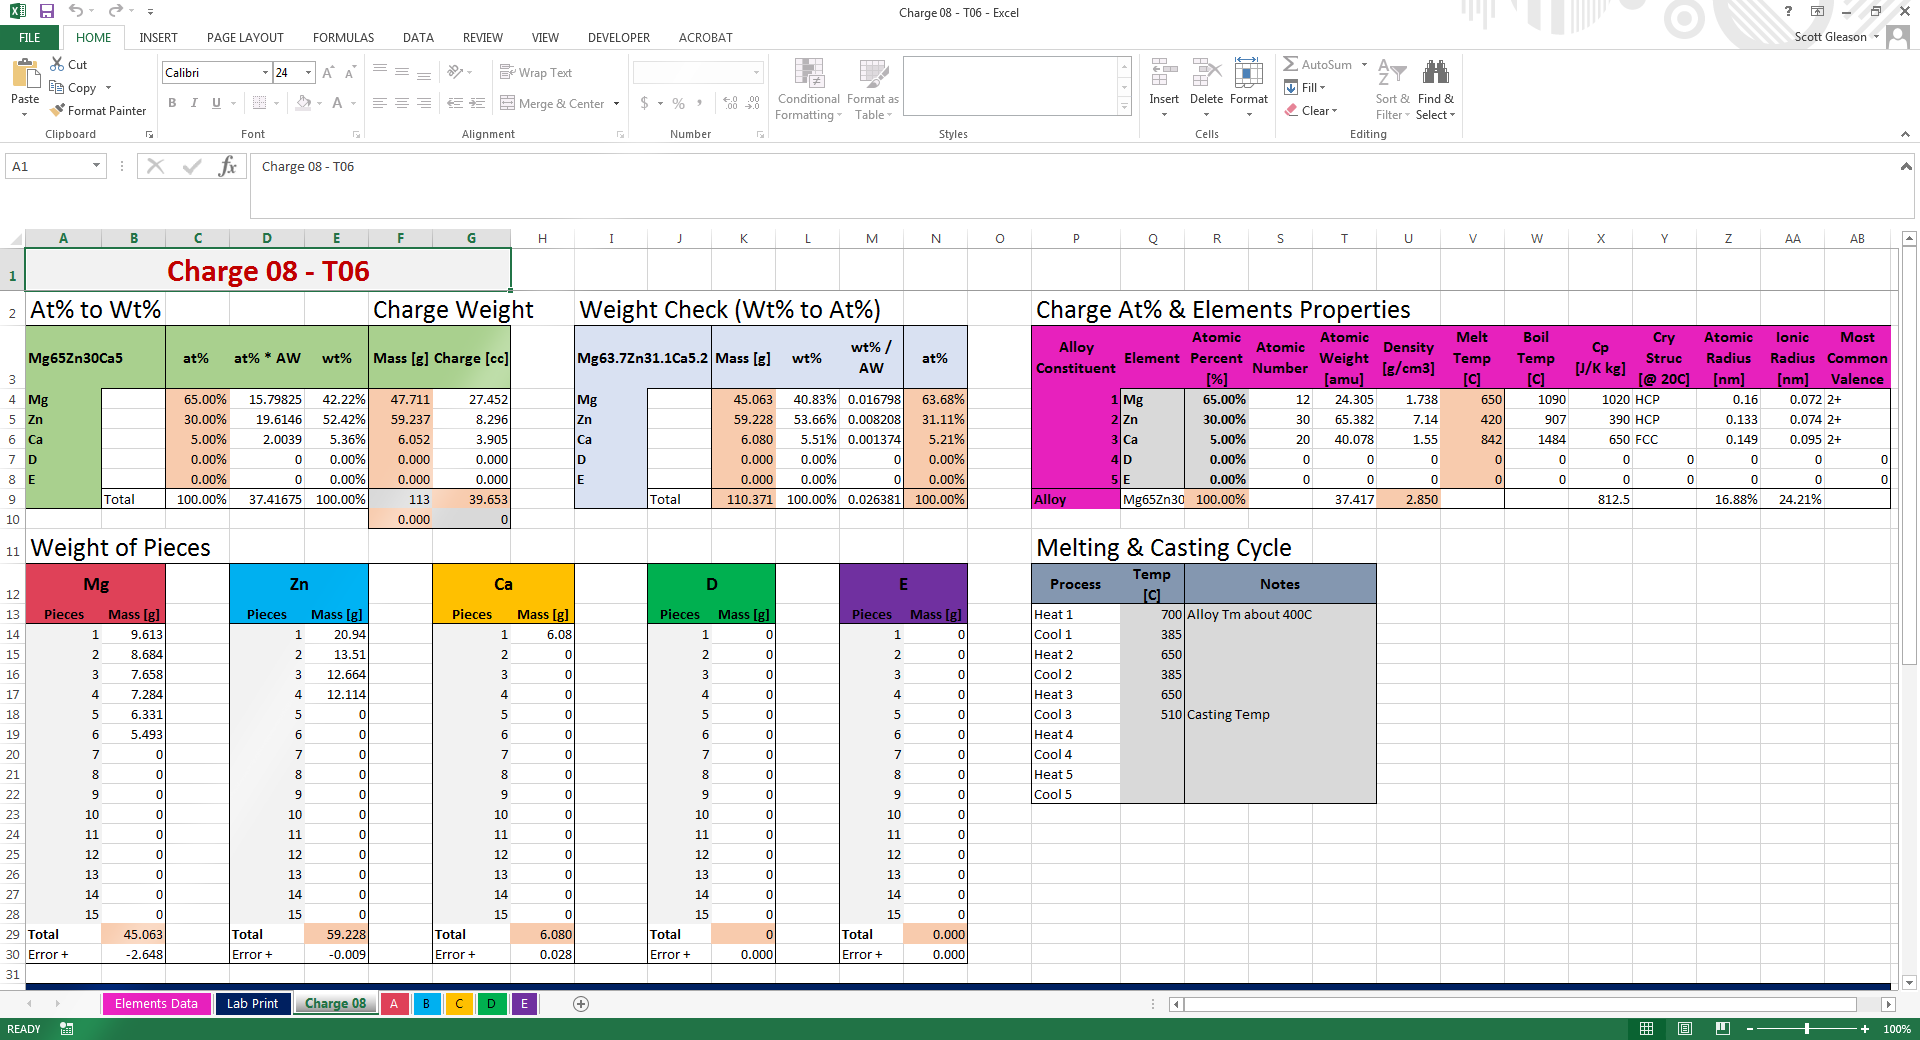
\includegraphics[width=0.99\textwidth]{Ex_ChargeSheet.png}
	\caption{Screenshot of the MS Excel workbook developed for auto-calculating master alloy charge weights, checking expected master alloy composition, and taking notes for future refinements.}
	\label{fig:ChargeSheet}
\end{figure}

\subsection{Induction Furnace}

The \MgZnCa~ master alloy was prepared from the base element ingots by an in house induction furnace and casting facility (Figures \ref{fig:CastingSchematic} and \ref{fig:LawsCasting}). The facility has a maximum temperature of 1300\degree C, heating rate of 500\degree C/min, and vacuum and dynamic gas melting capability \cite{Laws2007}. The dyanmic gas flow rate can be varied from $0-200~ cm^{3}/min$, and temperature regulated by a K-type thermocouple \cite{Laws2007}. The casting capabilities allow for conventional gravity casting, inverted injection casting, vacuum/suction casting or combination injection/vacuum casting \cite{Laws2007}.

%single image
\begin{figure}[htbp]
	\centering
	\includegraphics[width=0.75\textwidth]{Ex_Laws_Induction_Schematic.png}
	\caption[Schematic of induction casting melting chamber.]{Schematic of induction casting melting chamber. Adapted from \cite{Laws2007}.}
	\label{fig:CastingSchematic}
\end{figure}

The alloy was prepared with an in-house induction melting furnace within boron nitride coated graphite crucibles, purged with Ar (99.997 vol.\% purity) five times, and protected with a circulating Ar atmosphere. Alloy homogeneity was ensured by heating and cooling through a cycle of 700\degree C, 385\degree C, 650\degree C, 385\degree C, 650\degree C to a casting temperature of 500 \degree C and 450\degree C for injection and gravity casting respectively. Bulk amorphous \MgZnCa~ rods of nominal $2.5 mm$ diameter sectioned to $1mm$ thickness, and plates of nominal $1.2 mm$ thickness were produced by copper mold injection casting. The $25.4 mm$ diameter targets were prepared from cylindrical copper mold gravity castings sectioned to nominal thicknesses of $3.25mm$, and polished. All samples and targets were stored under Ar when not being examined or used. 

\subsection{Crucibles}

\subsection{Melt Cycle}

\subsection{Gravity Casting}

\subsection{Injection Casting}

\section{Bulk Sample Manufacture}

\subsection{Diamond Saw cutting}

\section{Semi-Crystalline Target Manufacture} 
test
\subsection{Induction Furnace}

\subsection{Melt Cycle}

\subsection{Gravity Casting}

\subsection{Riser Removal} 

\subsection{Target Extraction}

\subsection{Target Rounding}

\subsection{Target Polishing}

\section{Crystalline Target Manufacture}
test
\subsection{Induction Furnace}

\subsection{Melt Cycle}

\subsection{Gravity Casting}

\subsection{Sectioning of Targets}

\subsection{Target Rounding}

\subsection{Target Polishing}

\section{DC Magnetron Sputtering}
test
\subsection{DC Magnetron Sputtering}

\subsection{Deposition of Films}

\subsection{Target Lifespan}

\section{Examined Substrates} 
test
\subsection{Silicon Wafer Substrate}

\subsection{Silica Glass Substrate}

\subsection{Al DSC Lid Substrate}

\section{Storage}

\subsection{Desiccator}
Samples stored under Ar. 
10 - 15 purge cycles between 20 - 0 units. 
with moister beads in chamber. 
Samples kept within plastic bags inside of the dedicators. 

\section{Characterisation}
test
\subsection{Physical and Chemical Properties}

\subsection{Quality of Deposition} 
 
\subsection{Stylus profiler analysis}
Nominal film thickness was measure by a stylus profiler (Dektak 2A, Bruker, Germany). A glass slide was placed under the substrates within the sputtering chamber, allowing the substrates to act as a mask. Profile measurements were taken by measuring the height difference between the bare glass and the film coated glass. This film thickness was used to estimate the sputter deposition rate.  

\subsection{EDS analysis}
Alloy composition and homogeneity were confirmed by \acrshort{sem}-\acrshort{eds} (S3400-N, Hitachi, Japan; Nova NanoSEM 230/450, FEI, The Netherlands). Hyper-maps were collected with an accelerating voltage of $15-20keV$, a probe current of $50 \mu A$, spot size 4.2, counts of $5000cps$ or better, dead time less than 20\%, and working distance was $5mm$.

\subsection{DSC characterization}
Isochronic \acrshort{dsc} (204 F1 Phoenix, Netzsch, Selb, Germany) was carried out in Al crucibles under a protective Ar atmosphere (99.997 vol.\% purity). Scans were performed at \glspl{ht} of $5$ to $100 K/min$. 

Isothermal relaxation \acrshort{dsc} was preformed by heating samples at $20 K/min$ to the desired annealing temperature, holding for the desired time, and Ar quenching to room temperature.

For annealed \acrshort{xrd} the samples were heat treated in the \acrshort{dsc} by heating to the desired temperature at $20 K/min$ followed by Ar quenching to room temperature.

\subsection{XRD characterization}
Annealing \acrshort{xrd} (Empyrean, PANalytical, Cu $K_{\alpha}$ X-ray source, $\lambda = 1.541 \angstrom$) was performed on heat treated bulk rods and films at room temperature. 
With a generator voltage $45 kV$, tube current $40 mA$, scan step size 0.0262606, and time per step of 397.29. 

Dynamic \acrshort{xrd} (D8, Bruker, Cu $K_{\alpha}$ X-ray source, $\lambda = 1.541 \angstrom$) was performed on as manufactured bulk plates and films by raising temperature at a rate of $20 K/min$ and performing scans \textit{in situ}. The first scan was performed at $35$\degree C, then $75$\degree C, after which temperature was raised in $5$\degree C increments until reaching a final temperature at $185$\degree C. The $2 \theta$ scans from $31 - 60$\degree~ were completed within $1092 sec$ ($18min,~ 12sec$) to minimise the effects of recrystallisation during the experiment.
With a generator voltage $45 kV$, tube current $100 mA$, scan step size 0.02, and time per step of 134.4. 

%%%%%%%%%%%%%%%%%%%%%%%%%%%%%%%%%%%%%%%%%%%%%%%%%%%%%%%%%%%%%%%%%%%%%%%%%%

%Bibliography
\bibliography{ThesisBib}
\bibliographystyle{unsrt}

\end{document}